% Created by tikzDevice version 0.6.2-92-0ad2792 on 2013-03-28 14:53:09
% !TEX encoding = UTF-8 Unicode
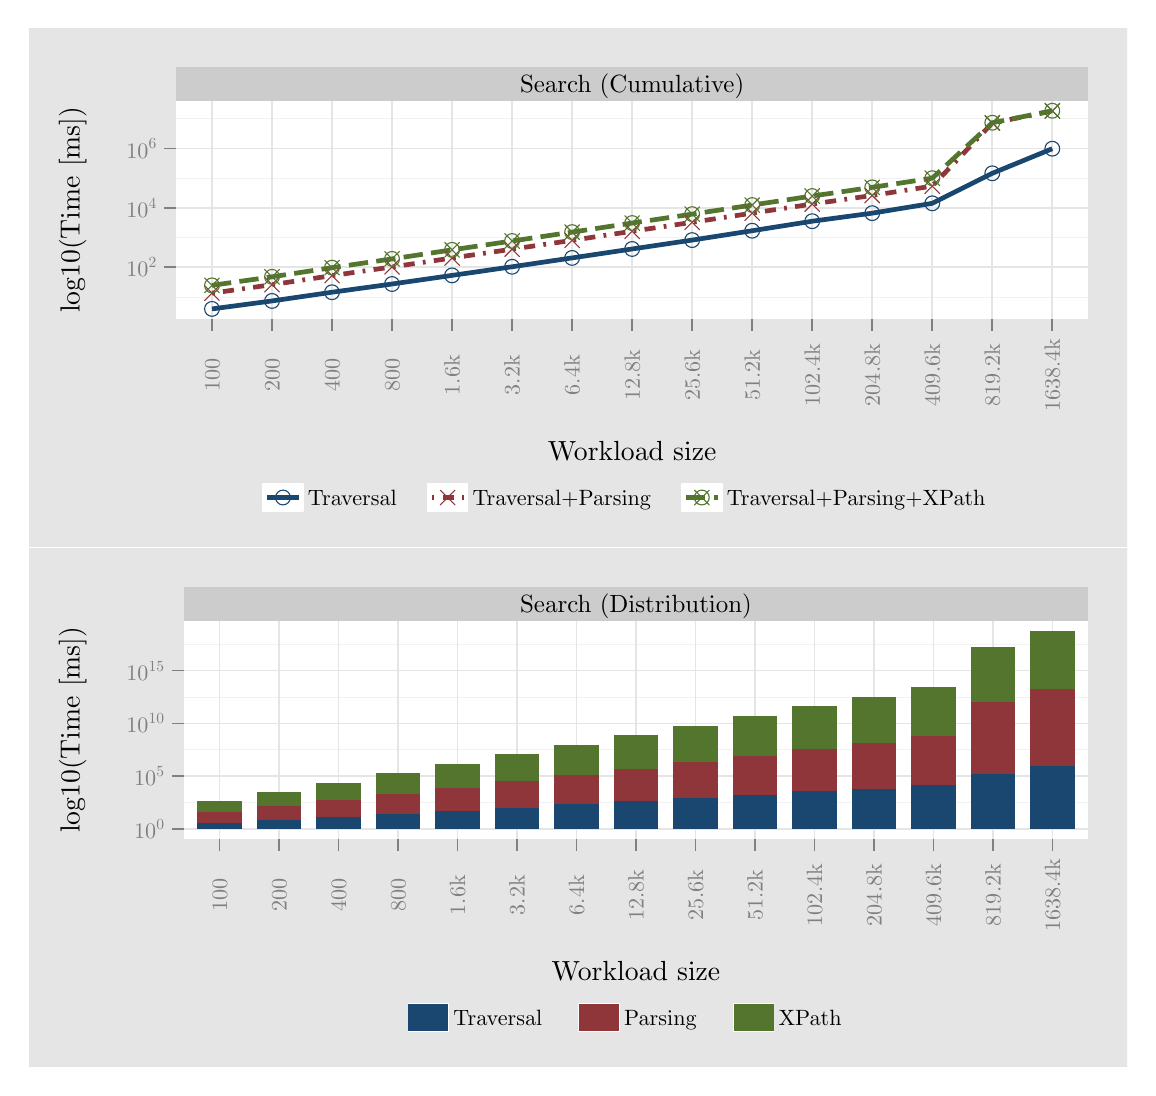
\begin{tikzpicture}[x=1pt,y=1pt]
\definecolor[named]{fillColor}{rgb}{1.00,1.00,1.00}
\path[use as bounding box,fill=fillColor,fill opacity=0.00] (0,0) rectangle (397.48,375.80);
\begin{scope}
\path[clip] (  0.00,187.90) rectangle (397.48,375.80);
\definecolor[named]{drawColor}{rgb}{1.00,1.00,1.00}
\definecolor[named]{fillColor}{rgb}{0.90,0.90,0.90}

\path[draw=drawColor,line width= 0.6pt,line join=round,line cap=round,fill=fillColor] (  0.00,187.90) rectangle (397.48,375.80);
\end{scope}
\begin{scope}
\path[clip] ( 53.58,270.59) rectangle (383.26,349.36);
\definecolor[named]{fillColor}{rgb}{1.00,1.00,1.00}

\path[fill=fillColor] ( 53.58,270.59) rectangle (383.26,349.36);
\definecolor[named]{drawColor}{rgb}{0.95,0.95,0.95}

\path[draw=drawColor,line width= 0.3pt,line join=round] ( 53.58,278.47) --
	(383.26,278.47);

\path[draw=drawColor,line width= 0.3pt,line join=round] ( 53.58,299.93) --
	(383.26,299.93);

\path[draw=drawColor,line width= 0.3pt,line join=round] ( 53.58,321.40) --
	(383.26,321.40);

\path[draw=drawColor,line width= 0.3pt,line join=round] ( 53.58,342.87) --
	(383.26,342.87);
\definecolor[named]{drawColor}{rgb}{0.90,0.90,0.90}

\path[draw=drawColor,line width= 0.6pt,line join=round] ( 53.58,289.20) --
	(383.26,289.20);

\path[draw=drawColor,line width= 0.6pt,line join=round] ( 53.58,310.67) --
	(383.26,310.67);

\path[draw=drawColor,line width= 0.6pt,line join=round] ( 53.58,332.13) --
	(383.26,332.13);

\path[draw=drawColor,line width= 0.6pt,line join=round] ( 66.60,270.59) --
	( 66.60,349.36);

\path[draw=drawColor,line width= 0.6pt,line join=round] ( 88.29,270.59) --
	( 88.29,349.36);

\path[draw=drawColor,line width= 0.6pt,line join=round] (109.97,270.59) --
	(109.97,349.36);

\path[draw=drawColor,line width= 0.6pt,line join=round] (131.66,270.59) --
	(131.66,349.36);

\path[draw=drawColor,line width= 0.6pt,line join=round] (153.35,270.59) --
	(153.35,349.36);

\path[draw=drawColor,line width= 0.6pt,line join=round] (175.04,270.59) --
	(175.04,349.36);

\path[draw=drawColor,line width= 0.6pt,line join=round] (196.73,270.59) --
	(196.73,349.36);

\path[draw=drawColor,line width= 0.6pt,line join=round] (218.42,270.59) --
	(218.42,349.36);

\path[draw=drawColor,line width= 0.6pt,line join=round] (240.11,270.59) --
	(240.11,349.36);

\path[draw=drawColor,line width= 0.6pt,line join=round] (261.80,270.59) --
	(261.80,349.36);

\path[draw=drawColor,line width= 0.6pt,line join=round] (283.49,270.59) --
	(283.49,349.36);

\path[draw=drawColor,line width= 0.6pt,line join=round] (305.18,270.59) --
	(305.18,349.36);

\path[draw=drawColor,line width= 0.6pt,line join=round] (326.87,270.59) --
	(326.87,349.36);

\path[draw=drawColor,line width= 0.6pt,line join=round] (348.56,270.59) --
	(348.56,349.36);

\path[draw=drawColor,line width= 0.6pt,line join=round] (370.25,270.59) --
	(370.25,349.36);
\definecolor[named]{drawColor}{rgb}{0.10,0.28,0.44}

\path[draw=drawColor,line width= 1.7pt,line join=round] ( 66.60,274.17) --
	( 88.29,277.05) --
	(109.97,280.20) --
	(131.66,283.17) --
	(153.35,286.28) --
	(175.04,289.40) --
	(196.73,292.60) --
	(218.42,295.83) --
	(240.11,299.04) --
	(261.80,302.42) --
	(283.49,305.86) --
	(305.18,308.77) --
	(326.87,312.32) --
	(348.56,323.17) --
	(370.25,332.06);
\definecolor[named]{drawColor}{rgb}{0.56,0.21,0.23}

\path[draw=drawColor,line width= 1.7pt,dash pattern=on 1pt off 3pt on 4pt off 3pt ,line join=round] ( 66.60,279.86) --
	( 88.29,282.93) --
	(109.97,286.20) --
	(131.66,289.34) --
	(153.35,292.57) --
	(175.04,295.76) --
	(196.73,298.95) --
	(218.42,302.23) --
	(240.11,305.47) --
	(261.80,308.78) --
	(283.49,312.06) --
	(305.18,315.16) --
	(326.87,318.55) --
	(348.56,341.33) --
	(370.25,345.69);
\definecolor[named]{drawColor}{rgb}{0.33,0.46,0.18}

\path[draw=drawColor,line width= 1.7pt,dash pattern=on 7pt off 3pt ,line join=round] ( 66.60,282.68) --
	( 88.29,285.77) --
	(109.97,289.08) --
	(131.66,292.24) --
	(153.35,295.51) --
	(175.04,298.71) --
	(196.73,301.92) --
	(218.42,305.20) --
	(240.11,308.42) --
	(261.80,311.70) --
	(283.49,314.96) --
	(305.18,318.10) --
	(326.87,321.41) --
	(348.56,341.44) --
	(370.25,345.78);
\definecolor[named]{drawColor}{rgb}{0.10,0.28,0.44}

\path[draw=drawColor,line width= 0.4pt,line join=round,line cap=round] ( 66.60,274.17) circle (  2.67);

\path[draw=drawColor,line width= 0.4pt,line join=round,line cap=round] ( 88.29,277.05) circle (  2.67);

\path[draw=drawColor,line width= 0.4pt,line join=round,line cap=round] (109.97,280.20) circle (  2.67);

\path[draw=drawColor,line width= 0.4pt,line join=round,line cap=round] (131.66,283.17) circle (  2.67);

\path[draw=drawColor,line width= 0.4pt,line join=round,line cap=round] (153.35,286.28) circle (  2.67);

\path[draw=drawColor,line width= 0.4pt,line join=round,line cap=round] (175.04,289.40) circle (  2.67);

\path[draw=drawColor,line width= 0.4pt,line join=round,line cap=round] (196.73,292.60) circle (  2.67);

\path[draw=drawColor,line width= 0.4pt,line join=round,line cap=round] (218.42,295.83) circle (  2.67);

\path[draw=drawColor,line width= 0.4pt,line join=round,line cap=round] (240.11,299.04) circle (  2.67);

\path[draw=drawColor,line width= 0.4pt,line join=round,line cap=round] (261.80,302.42) circle (  2.67);

\path[draw=drawColor,line width= 0.4pt,line join=round,line cap=round] (283.49,305.86) circle (  2.67);

\path[draw=drawColor,line width= 0.4pt,line join=round,line cap=round] (305.18,308.77) circle (  2.67);

\path[draw=drawColor,line width= 0.4pt,line join=round,line cap=round] (326.87,312.32) circle (  2.67);

\path[draw=drawColor,line width= 0.4pt,line join=round,line cap=round] (348.56,323.17) circle (  2.67);

\path[draw=drawColor,line width= 0.4pt,line join=round,line cap=round] (370.25,332.06) circle (  2.67);
\definecolor[named]{drawColor}{rgb}{0.56,0.21,0.23}

\path[draw=drawColor,line width= 0.4pt,line join=round,line cap=round,fill=fillColor] ( 63.93,277.19) -- ( 69.26,282.53);

\path[draw=drawColor,line width= 0.4pt,line join=round,line cap=round,fill=fillColor] ( 63.93,282.53) -- ( 69.26,277.19);

\path[draw=drawColor,line width= 0.4pt,line join=round,line cap=round,fill=fillColor] ( 85.62,280.27) -- ( 90.95,285.60);

\path[draw=drawColor,line width= 0.4pt,line join=round,line cap=round,fill=fillColor] ( 85.62,285.60) -- ( 90.95,280.27);

\path[draw=drawColor,line width= 0.4pt,line join=round,line cap=round,fill=fillColor] (107.31,283.53) -- (112.64,288.86);

\path[draw=drawColor,line width= 0.4pt,line join=round,line cap=round,fill=fillColor] (107.31,288.86) -- (112.64,283.53);

\path[draw=drawColor,line width= 0.4pt,line join=round,line cap=round,fill=fillColor] (129.00,286.68) -- (134.33,292.01);

\path[draw=drawColor,line width= 0.4pt,line join=round,line cap=round,fill=fillColor] (129.00,292.01) -- (134.33,286.68);

\path[draw=drawColor,line width= 0.4pt,line join=round,line cap=round,fill=fillColor] (150.69,289.90) -- (156.02,295.24);

\path[draw=drawColor,line width= 0.4pt,line join=round,line cap=round,fill=fillColor] (150.69,295.24) -- (156.02,289.90);

\path[draw=drawColor,line width= 0.4pt,line join=round,line cap=round,fill=fillColor] (172.37,293.09) -- (177.71,298.43);

\path[draw=drawColor,line width= 0.4pt,line join=round,line cap=round,fill=fillColor] (172.37,298.43) -- (177.71,293.09);

\path[draw=drawColor,line width= 0.4pt,line join=round,line cap=round,fill=fillColor] (194.06,296.29) -- (199.40,301.62);

\path[draw=drawColor,line width= 0.4pt,line join=round,line cap=round,fill=fillColor] (194.06,301.62) -- (199.40,296.29);

\path[draw=drawColor,line width= 0.4pt,line join=round,line cap=round,fill=fillColor] (215.75,299.56) -- (221.09,304.90);

\path[draw=drawColor,line width= 0.4pt,line join=round,line cap=round,fill=fillColor] (215.75,304.90) -- (221.09,299.56);

\path[draw=drawColor,line width= 0.4pt,line join=round,line cap=round,fill=fillColor] (237.44,302.80) -- (242.78,308.14);

\path[draw=drawColor,line width= 0.4pt,line join=round,line cap=round,fill=fillColor] (237.44,308.14) -- (242.78,302.80);

\path[draw=drawColor,line width= 0.4pt,line join=round,line cap=round,fill=fillColor] (259.13,306.11) -- (264.47,311.44);

\path[draw=drawColor,line width= 0.4pt,line join=round,line cap=round,fill=fillColor] (259.13,311.44) -- (264.47,306.11);

\path[draw=drawColor,line width= 0.4pt,line join=round,line cap=round,fill=fillColor] (280.82,309.39) -- (286.16,314.73);

\path[draw=drawColor,line width= 0.4pt,line join=round,line cap=round,fill=fillColor] (280.82,314.73) -- (286.16,309.39);

\path[draw=drawColor,line width= 0.4pt,line join=round,line cap=round,fill=fillColor] (302.51,312.49) -- (307.84,317.83);

\path[draw=drawColor,line width= 0.4pt,line join=round,line cap=round,fill=fillColor] (302.51,317.83) -- (307.84,312.49);

\path[draw=drawColor,line width= 0.4pt,line join=round,line cap=round,fill=fillColor] (324.20,315.88) -- (329.53,321.21);

\path[draw=drawColor,line width= 0.4pt,line join=round,line cap=round,fill=fillColor] (324.20,321.21) -- (329.53,315.88);

\path[draw=drawColor,line width= 0.4pt,line join=round,line cap=round,fill=fillColor] (345.89,338.66) -- (351.22,343.99);

\path[draw=drawColor,line width= 0.4pt,line join=round,line cap=round,fill=fillColor] (345.89,343.99) -- (351.22,338.66);

\path[draw=drawColor,line width= 0.4pt,line join=round,line cap=round,fill=fillColor] (367.58,343.02) -- (372.91,348.36);

\path[draw=drawColor,line width= 0.4pt,line join=round,line cap=round,fill=fillColor] (367.58,348.36) -- (372.91,343.02);
\definecolor[named]{drawColor}{rgb}{0.33,0.46,0.18}

\path[draw=drawColor,line width= 0.4pt,line join=round,line cap=round] ( 66.60,282.68) circle (  2.67);

\path[draw=drawColor,line width= 0.4pt,line join=round,line cap=round] ( 63.93,280.01) -- ( 69.26,285.34);

\path[draw=drawColor,line width= 0.4pt,line join=round,line cap=round] ( 63.93,285.34) -- ( 69.26,280.01);

\path[draw=drawColor,line width= 0.4pt,line join=round,line cap=round] ( 88.29,285.77) circle (  2.67);

\path[draw=drawColor,line width= 0.4pt,line join=round,line cap=round] ( 85.62,283.10) -- ( 90.95,288.44);

\path[draw=drawColor,line width= 0.4pt,line join=round,line cap=round] ( 85.62,288.44) -- ( 90.95,283.10);

\path[draw=drawColor,line width= 0.4pt,line join=round,line cap=round] (109.97,289.08) circle (  2.67);

\path[draw=drawColor,line width= 0.4pt,line join=round,line cap=round] (107.31,286.41) -- (112.64,291.75);

\path[draw=drawColor,line width= 0.4pt,line join=round,line cap=round] (107.31,291.75) -- (112.64,286.41);

\path[draw=drawColor,line width= 0.4pt,line join=round,line cap=round] (131.66,292.24) circle (  2.67);

\path[draw=drawColor,line width= 0.4pt,line join=round,line cap=round] (129.00,289.57) -- (134.33,294.91);

\path[draw=drawColor,line width= 0.4pt,line join=round,line cap=round] (129.00,294.91) -- (134.33,289.57);

\path[draw=drawColor,line width= 0.4pt,line join=round,line cap=round] (153.35,295.51) circle (  2.67);

\path[draw=drawColor,line width= 0.4pt,line join=round,line cap=round] (150.69,292.84) -- (156.02,298.18);

\path[draw=drawColor,line width= 0.4pt,line join=round,line cap=round] (150.69,298.18) -- (156.02,292.84);

\path[draw=drawColor,line width= 0.4pt,line join=round,line cap=round] (175.04,298.71) circle (  2.67);

\path[draw=drawColor,line width= 0.4pt,line join=round,line cap=round] (172.37,296.04) -- (177.71,301.37);

\path[draw=drawColor,line width= 0.4pt,line join=round,line cap=round] (172.37,301.37) -- (177.71,296.04);

\path[draw=drawColor,line width= 0.4pt,line join=round,line cap=round] (196.73,301.92) circle (  2.67);

\path[draw=drawColor,line width= 0.4pt,line join=round,line cap=round] (194.06,299.25) -- (199.40,304.59);

\path[draw=drawColor,line width= 0.4pt,line join=round,line cap=round] (194.06,304.59) -- (199.40,299.25);

\path[draw=drawColor,line width= 0.4pt,line join=round,line cap=round] (218.42,305.20) circle (  2.67);

\path[draw=drawColor,line width= 0.4pt,line join=round,line cap=round] (215.75,302.53) -- (221.09,307.87);

\path[draw=drawColor,line width= 0.4pt,line join=round,line cap=round] (215.75,307.87) -- (221.09,302.53);

\path[draw=drawColor,line width= 0.4pt,line join=round,line cap=round] (240.11,308.42) circle (  2.67);

\path[draw=drawColor,line width= 0.4pt,line join=round,line cap=round] (237.44,305.75) -- (242.78,311.09);

\path[draw=drawColor,line width= 0.4pt,line join=round,line cap=round] (237.44,311.09) -- (242.78,305.75);

\path[draw=drawColor,line width= 0.4pt,line join=round,line cap=round] (261.80,311.70) circle (  2.67);

\path[draw=drawColor,line width= 0.4pt,line join=round,line cap=round] (259.13,309.04) -- (264.47,314.37);

\path[draw=drawColor,line width= 0.4pt,line join=round,line cap=round] (259.13,314.37) -- (264.47,309.04);

\path[draw=drawColor,line width= 0.4pt,line join=round,line cap=round] (283.49,314.96) circle (  2.67);

\path[draw=drawColor,line width= 0.4pt,line join=round,line cap=round] (280.82,312.29) -- (286.16,317.63);

\path[draw=drawColor,line width= 0.4pt,line join=round,line cap=round] (280.82,317.63) -- (286.16,312.29);

\path[draw=drawColor,line width= 0.4pt,line join=round,line cap=round] (305.18,318.10) circle (  2.67);

\path[draw=drawColor,line width= 0.4pt,line join=round,line cap=round] (302.51,315.44) -- (307.84,320.77);

\path[draw=drawColor,line width= 0.4pt,line join=round,line cap=round] (302.51,320.77) -- (307.84,315.44);

\path[draw=drawColor,line width= 0.4pt,line join=round,line cap=round] (326.87,321.41) circle (  2.67);

\path[draw=drawColor,line width= 0.4pt,line join=round,line cap=round] (324.20,318.75) -- (329.53,324.08);

\path[draw=drawColor,line width= 0.4pt,line join=round,line cap=round] (324.20,324.08) -- (329.53,318.75);

\path[draw=drawColor,line width= 0.4pt,line join=round,line cap=round] (348.56,341.44) circle (  2.67);

\path[draw=drawColor,line width= 0.4pt,line join=round,line cap=round] (345.89,338.77) -- (351.22,344.11);

\path[draw=drawColor,line width= 0.4pt,line join=round,line cap=round] (345.89,344.11) -- (351.22,338.77);

\path[draw=drawColor,line width= 0.4pt,line join=round,line cap=round] (370.25,345.78) circle (  2.67);

\path[draw=drawColor,line width= 0.4pt,line join=round,line cap=round] (367.58,343.11) -- (372.91,348.44);

\path[draw=drawColor,line width= 0.4pt,line join=round,line cap=round] (367.58,348.44) -- (372.91,343.11);
\end{scope}
\begin{scope}
\path[clip] (  0.00,  0.00) rectangle (397.48,375.80);
\definecolor[named]{fillColor}{rgb}{0.80,0.80,0.80}

\path[fill=fillColor] ( 53.58,349.36) rectangle (383.26,361.58);
\definecolor[named]{drawColor}{rgb}{0.00,0.00,0.00}

\node[text=drawColor,anchor=base,inner sep=0pt, outer sep=0pt, scale=  0.90] at (218.42,352.37) {Search (Cumulative)};
\end{scope}
\begin{scope}
\path[clip] (  0.00,  0.00) rectangle (397.48,375.80);
\definecolor[named]{drawColor}{rgb}{0.50,0.50,0.50}

\node[text=drawColor,anchor=base west,inner sep=0pt, outer sep=0pt, scale=  0.80] at ( 35.67,285.77) {10};

\node[text=drawColor,anchor=base west,inner sep=0pt, outer sep=0pt, scale=  0.56] at ( 43.67,289.04) {2};

\node[text=drawColor,anchor=base west,inner sep=0pt, outer sep=0pt, scale=  0.80] at ( 35.67,307.24) {10};

\node[text=drawColor,anchor=base west,inner sep=0pt, outer sep=0pt, scale=  0.56] at ( 43.67,310.51) {4};

\node[text=drawColor,anchor=base west,inner sep=0pt, outer sep=0pt, scale=  0.80] at ( 35.67,328.70) {10};

\node[text=drawColor,anchor=base west,inner sep=0pt, outer sep=0pt, scale=  0.56] at ( 43.67,331.97) {6};
\end{scope}
\begin{scope}
\path[clip] (  0.00,  0.00) rectangle (397.48,375.80);
\definecolor[named]{drawColor}{rgb}{0.50,0.50,0.50}

\path[draw=drawColor,line width= 0.6pt,line join=round] ( 49.31,289.20) --
	( 53.58,289.20);

\path[draw=drawColor,line width= 0.6pt,line join=round] ( 49.31,310.67) --
	( 53.58,310.67);

\path[draw=drawColor,line width= 0.6pt,line join=round] ( 49.31,332.13) --
	( 53.58,332.13);
\end{scope}
\begin{scope}
\path[clip] (  0.00,  0.00) rectangle (397.48,375.80);
\definecolor[named]{drawColor}{rgb}{0.50,0.50,0.50}

\path[draw=drawColor,line width= 0.6pt,line join=round] ( 66.60,266.32) --
	( 66.60,270.59);

\path[draw=drawColor,line width= 0.6pt,line join=round] ( 88.29,266.32) --
	( 88.29,270.59);

\path[draw=drawColor,line width= 0.6pt,line join=round] (109.97,266.32) --
	(109.97,270.59);

\path[draw=drawColor,line width= 0.6pt,line join=round] (131.66,266.32) --
	(131.66,270.59);

\path[draw=drawColor,line width= 0.6pt,line join=round] (153.35,266.32) --
	(153.35,270.59);

\path[draw=drawColor,line width= 0.6pt,line join=round] (175.04,266.32) --
	(175.04,270.59);

\path[draw=drawColor,line width= 0.6pt,line join=round] (196.73,266.32) --
	(196.73,270.59);

\path[draw=drawColor,line width= 0.6pt,line join=round] (218.42,266.32) --
	(218.42,270.59);

\path[draw=drawColor,line width= 0.6pt,line join=round] (240.11,266.32) --
	(240.11,270.59);

\path[draw=drawColor,line width= 0.6pt,line join=round] (261.80,266.32) --
	(261.80,270.59);

\path[draw=drawColor,line width= 0.6pt,line join=round] (283.49,266.32) --
	(283.49,270.59);

\path[draw=drawColor,line width= 0.6pt,line join=round] (305.18,266.32) --
	(305.18,270.59);

\path[draw=drawColor,line width= 0.6pt,line join=round] (326.87,266.32) --
	(326.87,270.59);

\path[draw=drawColor,line width= 0.6pt,line join=round] (348.56,266.32) --
	(348.56,270.59);

\path[draw=drawColor,line width= 0.6pt,line join=round] (370.25,266.32) --
	(370.25,270.59);
\end{scope}
\begin{scope}
\path[clip] (  0.00,  0.00) rectangle (397.48,375.80);
\definecolor[named]{drawColor}{rgb}{0.50,0.50,0.50}

\node[text=drawColor,rotate= 90.00,anchor=base,inner sep=0pt, outer sep=0pt, scale=  0.80] at ( 69.35,250.26) {100};

\node[text=drawColor,rotate= 90.00,anchor=base,inner sep=0pt, outer sep=0pt, scale=  0.80] at ( 91.04,250.26) {200};

\node[text=drawColor,rotate= 90.00,anchor=base,inner sep=0pt, outer sep=0pt, scale=  0.80] at (112.73,250.26) {400};

\node[text=drawColor,rotate= 90.00,anchor=base,inner sep=0pt, outer sep=0pt, scale=  0.80] at (134.42,250.26) {800};

\node[text=drawColor,rotate= 90.00,anchor=base,inner sep=0pt, outer sep=0pt, scale=  0.80] at (156.11,250.26) {1.6k};

\node[text=drawColor,rotate= 90.00,anchor=base,inner sep=0pt, outer sep=0pt, scale=  0.80] at (177.80,250.26) {3.2k};

\node[text=drawColor,rotate= 90.00,anchor=base,inner sep=0pt, outer sep=0pt, scale=  0.80] at (199.49,250.26) {6.4k};

\node[text=drawColor,rotate= 90.00,anchor=base,inner sep=0pt, outer sep=0pt, scale=  0.80] at (221.18,250.26) {12.8k};

\node[text=drawColor,rotate= 90.00,anchor=base,inner sep=0pt, outer sep=0pt, scale=  0.80] at (242.86,250.26) {25.6k};

\node[text=drawColor,rotate= 90.00,anchor=base,inner sep=0pt, outer sep=0pt, scale=  0.80] at (264.55,250.26) {51.2k};

\node[text=drawColor,rotate= 90.00,anchor=base,inner sep=0pt, outer sep=0pt, scale=  0.80] at (286.24,250.26) {102.4k};

\node[text=drawColor,rotate= 90.00,anchor=base,inner sep=0pt, outer sep=0pt, scale=  0.80] at (307.93,250.26) {204.8k};

\node[text=drawColor,rotate= 90.00,anchor=base,inner sep=0pt, outer sep=0pt, scale=  0.80] at (329.62,250.26) {409.6k};

\node[text=drawColor,rotate= 90.00,anchor=base,inner sep=0pt, outer sep=0pt, scale=  0.80] at (351.31,250.26) {819.2k};

\node[text=drawColor,rotate= 90.00,anchor=base,inner sep=0pt, outer sep=0pt, scale=  0.80] at (373.00,250.26) {1638.4k};
\end{scope}
\begin{scope}
\path[clip] (  0.00,  0.00) rectangle (397.48,375.80);
\definecolor[named]{drawColor}{rgb}{0.00,0.00,0.00}

\node[text=drawColor,anchor=base,inner sep=0pt, outer sep=0pt, scale=  1.00] at (218.42,219.31) {Workload size};
\end{scope}
\begin{scope}
\path[clip] (  0.00,  0.00) rectangle (397.48,375.80);
\definecolor[named]{drawColor}{rgb}{0.00,0.00,0.00}

\node[text=drawColor,rotate= 90.00,anchor=base,inner sep=0pt, outer sep=0pt, scale=  1.00] at ( 18.80,309.97) {log10(Time [ms])};
\end{scope}
\begin{scope}
\path[clip] (  0.00,  0.00) rectangle (397.48,375.80);
\definecolor[named]{fillColor}{rgb}{0.90,0.90,0.90}

\path[fill=fillColor] ( 77.14,196.77) rectangle (359.70,215.26);
\end{scope}
\begin{scope}
\path[clip] (  0.00,  0.00) rectangle (397.48,375.80);
\definecolor[named]{drawColor}{rgb}{1.00,1.00,1.00}
\definecolor[named]{fillColor}{rgb}{1.00,1.00,1.00}

\path[draw=drawColor,line width= 0.6pt,line join=round,line cap=round,fill=fillColor] ( 85.02,201.04) rectangle ( 99.47,211.00);
\end{scope}
\begin{scope}
\path[clip] (  0.00,  0.00) rectangle (397.48,375.80);
\definecolor[named]{drawColor}{rgb}{0.10,0.28,0.44}

\path[draw=drawColor,line width= 1.7pt,line join=round] ( 86.47,206.02) -- ( 98.03,206.02);
\end{scope}
\begin{scope}
\path[clip] (  0.00,  0.00) rectangle (397.48,375.80);
\definecolor[named]{drawColor}{rgb}{0.10,0.28,0.44}

\path[draw=drawColor,line width= 0.4pt,line join=round,line cap=round] ( 92.25,206.02) circle (  2.67);
\end{scope}
\begin{scope}
\path[clip] (  0.00,  0.00) rectangle (397.48,375.80);
\definecolor[named]{drawColor}{rgb}{1.00,1.00,1.00}
\definecolor[named]{fillColor}{rgb}{1.00,1.00,1.00}

\path[draw=drawColor,line width= 0.6pt,line join=round,line cap=round,fill=fillColor] (144.50,201.04) rectangle (158.96,211.00);
\end{scope}
\begin{scope}
\path[clip] (  0.00,  0.00) rectangle (397.48,375.80);
\definecolor[named]{drawColor}{rgb}{0.56,0.21,0.23}

\path[draw=drawColor,line width= 1.7pt,dash pattern=on 1pt off 3pt on 4pt off 3pt ,line join=round] (145.95,206.02) -- (157.51,206.02);
\end{scope}
\begin{scope}
\path[clip] (  0.00,  0.00) rectangle (397.48,375.80);
\definecolor[named]{drawColor}{rgb}{0.56,0.21,0.23}
\definecolor[named]{fillColor}{rgb}{1.00,1.00,1.00}

\path[draw=drawColor,line width= 0.4pt,line join=round,line cap=round,fill=fillColor] (149.06,203.35) -- (154.40,208.68);

\path[draw=drawColor,line width= 0.4pt,line join=round,line cap=round,fill=fillColor] (149.06,208.68) -- (154.40,203.35);
\end{scope}
\begin{scope}
\path[clip] (  0.00,  0.00) rectangle (397.48,375.80);
\definecolor[named]{drawColor}{rgb}{1.00,1.00,1.00}
\definecolor[named]{fillColor}{rgb}{1.00,1.00,1.00}

\path[draw=drawColor,line width= 0.6pt,line join=round,line cap=round,fill=fillColor] (236.37,201.04) rectangle (250.83,211.00);
\end{scope}
\begin{scope}
\path[clip] (  0.00,  0.00) rectangle (397.48,375.80);
\definecolor[named]{drawColor}{rgb}{0.33,0.46,0.18}

\path[draw=drawColor,line width= 1.7pt,dash pattern=on 7pt off 3pt ,line join=round] (237.82,206.02) -- (249.38,206.02);
\end{scope}
\begin{scope}
\path[clip] (  0.00,  0.00) rectangle (397.48,375.80);
\definecolor[named]{drawColor}{rgb}{0.33,0.46,0.18}

\path[draw=drawColor,line width= 0.4pt,line join=round,line cap=round] (243.60,206.02) circle (  2.67);

\path[draw=drawColor,line width= 0.4pt,line join=round,line cap=round] (240.93,203.35) -- (246.27,208.68);

\path[draw=drawColor,line width= 0.4pt,line join=round,line cap=round] (240.93,208.68) -- (246.27,203.35);
\end{scope}
\begin{scope}
\path[clip] (  0.00,  0.00) rectangle (397.48,375.80);
\definecolor[named]{drawColor}{rgb}{0.00,0.00,0.00}

\node[text=drawColor,anchor=base west,inner sep=0pt, outer sep=0pt, scale=  0.80] at (101.28,203.26) {Traversal $\;\;\;$};
\end{scope}
\begin{scope}
\path[clip] (  0.00,  0.00) rectangle (397.48,375.80);
\definecolor[named]{drawColor}{rgb}{0.00,0.00,0.00}

\node[text=drawColor,anchor=base west,inner sep=0pt, outer sep=0pt, scale=  0.80] at (160.76,203.26) {Traversal+Parsing $\;\;\;$};
\end{scope}
\begin{scope}
\path[clip] (  0.00,  0.00) rectangle (397.48,375.80);
\definecolor[named]{drawColor}{rgb}{0.00,0.00,0.00}

\node[text=drawColor,anchor=base west,inner sep=0pt, outer sep=0pt, scale=  0.80] at (252.64,203.26) {Traversal+Parsing+XPath $\;\;\;$};
\end{scope}
\begin{scope}
\path[clip] (  0.00,  0.00) rectangle (397.48,187.90);
\definecolor[named]{drawColor}{rgb}{1.00,1.00,1.00}
\definecolor[named]{fillColor}{rgb}{0.90,0.90,0.90}

\path[draw=drawColor,line width= 0.6pt,line join=round,line cap=round,fill=fillColor] (  0.00,  0.00) rectangle (397.48,187.90);
\end{scope}
\begin{scope}
\path[clip] ( 56.38, 82.69) rectangle (383.26,161.45);
\definecolor[named]{fillColor}{rgb}{1.00,1.00,1.00}

\path[fill=fillColor] ( 56.38, 82.69) rectangle (383.26,161.45);
\definecolor[named]{drawColor}{rgb}{0.95,0.95,0.95}

\path[draw=drawColor,line width= 0.3pt,line join=round] ( 56.38, 95.81) --
	(383.26, 95.81);

\path[draw=drawColor,line width= 0.3pt,line join=round] ( 56.38,114.88) --
	(383.26,114.88);

\path[draw=drawColor,line width= 0.3pt,line join=round] ( 56.38,133.96) --
	(383.26,133.96);

\path[draw=drawColor,line width= 0.3pt,line join=round] ( 56.38,153.03) --
	(383.26,153.03);
\definecolor[named]{drawColor}{rgb}{0.90,0.90,0.90}

\path[draw=drawColor,line width= 0.6pt,line join=round] ( 56.38, 86.27) --
	(383.26, 86.27);

\path[draw=drawColor,line width= 0.6pt,line join=round] ( 56.38,105.34) --
	(383.26,105.34);

\path[draw=drawColor,line width= 0.6pt,line join=round] ( 56.38,124.42) --
	(383.26,124.42);

\path[draw=drawColor,line width= 0.6pt,line join=round] ( 56.38,143.49) --
	(383.26,143.49);

\path[draw=drawColor,line width= 0.6pt,line join=round] ( 69.28, 82.69) --
	( 69.28,161.45);

\path[draw=drawColor,line width= 0.6pt,line join=round] ( 90.79, 82.69) --
	( 90.79,161.45);

\path[draw=drawColor,line width= 0.6pt,line join=round] (112.29, 82.69) --
	(112.29,161.45);

\path[draw=drawColor,line width= 0.6pt,line join=round] (133.80, 82.69) --
	(133.80,161.45);

\path[draw=drawColor,line width= 0.6pt,line join=round] (155.31, 82.69) --
	(155.31,161.45);

\path[draw=drawColor,line width= 0.6pt,line join=round] (176.81, 82.69) --
	(176.81,161.45);

\path[draw=drawColor,line width= 0.6pt,line join=round] (198.32, 82.69) --
	(198.32,161.45);

\path[draw=drawColor,line width= 0.6pt,line join=round] (219.82, 82.69) --
	(219.82,161.45);

\path[draw=drawColor,line width= 0.6pt,line join=round] (241.33, 82.69) --
	(241.33,161.45);

\path[draw=drawColor,line width= 0.6pt,line join=round] (262.83, 82.69) --
	(262.83,161.45);

\path[draw=drawColor,line width= 0.6pt,line join=round] (284.34, 82.69) --
	(284.34,161.45);

\path[draw=drawColor,line width= 0.6pt,line join=round] (305.84, 82.69) --
	(305.84,161.45);

\path[draw=drawColor,line width= 0.6pt,line join=round] (327.35, 82.69) --
	(327.35,161.45);

\path[draw=drawColor,line width= 0.6pt,line join=round] (348.85, 82.69) --
	(348.85,161.45);

\path[draw=drawColor,line width= 0.6pt,line join=round] (370.36, 82.69) --
	(370.36,161.45);
\definecolor[named]{fillColor}{rgb}{0.10,0.28,0.44}

\path[fill=fillColor] ( 61.22, 86.27) rectangle ( 77.35, 88.56);
\definecolor[named]{fillColor}{rgb}{0.56,0.21,0.23}

\path[fill=fillColor] ( 61.22, 88.56) rectangle ( 77.35, 92.29);
\definecolor[named]{fillColor}{rgb}{0.33,0.46,0.18}

\path[fill=fillColor] ( 61.22, 92.29) rectangle ( 77.35, 96.29);
\definecolor[named]{fillColor}{rgb}{0.10,0.28,0.44}

\path[fill=fillColor] ( 82.73, 86.27) rectangle ( 98.85, 89.58);
\definecolor[named]{fillColor}{rgb}{0.56,0.21,0.23}

\path[fill=fillColor] ( 82.73, 89.58) rectangle ( 98.85, 94.43);
\definecolor[named]{fillColor}{rgb}{0.33,0.46,0.18}

\path[fill=fillColor] ( 82.73, 94.43) rectangle ( 98.85, 99.54);
\definecolor[named]{fillColor}{rgb}{0.10,0.28,0.44}

\path[fill=fillColor] (104.23, 86.27) rectangle (120.36, 90.70);
\definecolor[named]{fillColor}{rgb}{0.56,0.21,0.23}

\path[fill=fillColor] (104.23, 90.70) rectangle (120.36, 96.73);
\definecolor[named]{fillColor}{rgb}{0.33,0.46,0.18}

\path[fill=fillColor] (104.23, 96.73) rectangle (120.36,103.03);
\definecolor[named]{fillColor}{rgb}{0.10,0.28,0.44}

\path[fill=fillColor] (125.74, 86.27) rectangle (141.86, 91.76);
\definecolor[named]{fillColor}{rgb}{0.56,0.21,0.23}

\path[fill=fillColor] (125.74, 91.76) rectangle (141.86, 98.92);
\definecolor[named]{fillColor}{rgb}{0.33,0.46,0.18}

\path[fill=fillColor] (125.74, 98.92) rectangle (141.86,106.36);
\definecolor[named]{fillColor}{rgb}{0.10,0.28,0.44}

\path[fill=fillColor] (147.24, 86.27) rectangle (163.37, 92.86);
\definecolor[named]{fillColor}{rgb}{0.56,0.21,0.23}

\path[fill=fillColor] (147.24, 92.86) rectangle (163.37,101.19);
\definecolor[named]{fillColor}{rgb}{0.33,0.46,0.18}

\path[fill=fillColor] (147.24,101.19) rectangle (163.37,109.80);
\definecolor[named]{fillColor}{rgb}{0.10,0.28,0.44}

\path[fill=fillColor] (168.75, 86.27) rectangle (184.87, 93.97);
\definecolor[named]{fillColor}{rgb}{0.56,0.21,0.23}

\path[fill=fillColor] (168.75, 93.97) rectangle (184.87,103.44);
\definecolor[named]{fillColor}{rgb}{0.33,0.46,0.18}

\path[fill=fillColor] (168.75,103.44) rectangle (184.87,113.19);
\definecolor[named]{fillColor}{rgb}{0.10,0.28,0.44}

\path[fill=fillColor] (190.25, 86.27) rectangle (206.38, 95.11);
\definecolor[named]{fillColor}{rgb}{0.56,0.21,0.23}

\path[fill=fillColor] (190.25, 95.11) rectangle (206.38,105.72);
\definecolor[named]{fillColor}{rgb}{0.33,0.46,0.18}

\path[fill=fillColor] (190.25,105.72) rectangle (206.38,116.62);
\definecolor[named]{fillColor}{rgb}{0.10,0.28,0.44}

\path[fill=fillColor] (211.76, 86.27) rectangle (227.88, 96.26);
\definecolor[named]{fillColor}{rgb}{0.56,0.21,0.23}

\path[fill=fillColor] (211.76, 96.26) rectangle (227.88,108.03);
\definecolor[named]{fillColor}{rgb}{0.33,0.46,0.18}

\path[fill=fillColor] (211.76,108.03) rectangle (227.88,120.10);
\definecolor[named]{fillColor}{rgb}{0.10,0.28,0.44}

\path[fill=fillColor] (233.26, 86.27) rectangle (249.39, 97.40);
\definecolor[named]{fillColor}{rgb}{0.56,0.21,0.23}

\path[fill=fillColor] (233.26, 97.40) rectangle (249.39,110.33);
\definecolor[named]{fillColor}{rgb}{0.33,0.46,0.18}

\path[fill=fillColor] (233.26,110.33) rectangle (249.39,123.53);
\definecolor[named]{fillColor}{rgb}{0.10,0.28,0.44}

\path[fill=fillColor] (254.77, 86.27) rectangle (270.89, 98.60);
\definecolor[named]{fillColor}{rgb}{0.56,0.21,0.23}

\path[fill=fillColor] (254.77, 98.60) rectangle (270.89,112.70);
\definecolor[named]{fillColor}{rgb}{0.33,0.46,0.18}

\path[fill=fillColor] (254.77,112.70) rectangle (270.89,127.06);
\definecolor[named]{fillColor}{rgb}{0.10,0.28,0.44}

\path[fill=fillColor] (276.27, 86.27) rectangle (292.40, 99.82);
\definecolor[named]{fillColor}{rgb}{0.56,0.21,0.23}

\path[fill=fillColor] (276.27, 99.82) rectangle (292.40,115.07);
\definecolor[named]{fillColor}{rgb}{0.33,0.46,0.18}

\path[fill=fillColor] (276.27,115.07) rectangle (292.40,130.57);
\definecolor[named]{fillColor}{rgb}{0.10,0.28,0.44}

\path[fill=fillColor] (297.78, 86.27) rectangle (313.90,100.86);
\definecolor[named]{fillColor}{rgb}{0.56,0.21,0.23}

\path[fill=fillColor] (297.78,100.86) rectangle (313.90,117.23);
\definecolor[named]{fillColor}{rgb}{0.33,0.46,0.18}

\path[fill=fillColor] (297.78,117.23) rectangle (313.90,133.87);
\definecolor[named]{fillColor}{rgb}{0.10,0.28,0.44}

\path[fill=fillColor] (319.28, 86.27) rectangle (335.41,102.12);
\definecolor[named]{fillColor}{rgb}{0.56,0.21,0.23}

\path[fill=fillColor] (319.28,102.12) rectangle (335.41,119.67);
\definecolor[named]{fillColor}{rgb}{0.33,0.46,0.18}

\path[fill=fillColor] (319.28,119.67) rectangle (335.41,137.46);
\definecolor[named]{fillColor}{rgb}{0.10,0.28,0.44}

\path[fill=fillColor] (340.79, 86.27) rectangle (356.91,105.98);
\definecolor[named]{fillColor}{rgb}{0.56,0.21,0.23}

\path[fill=fillColor] (340.79,105.98) rectangle (356.91,132.10);
\definecolor[named]{fillColor}{rgb}{0.33,0.46,0.18}

\path[fill=fillColor] (340.79,132.10) rectangle (356.91,152.14);
\definecolor[named]{fillColor}{rgb}{0.10,0.28,0.44}

\path[fill=fillColor] (362.29, 86.27) rectangle (378.42,109.13);
\definecolor[named]{fillColor}{rgb}{0.56,0.21,0.23}

\path[fill=fillColor] (362.29,109.13) rectangle (378.42,136.75);
\definecolor[named]{fillColor}{rgb}{0.33,0.46,0.18}

\path[fill=fillColor] (362.29,136.75) rectangle (378.42,157.87);
\end{scope}
\begin{scope}
\path[clip] (  0.00,  0.00) rectangle (397.48,375.80);
\definecolor[named]{fillColor}{rgb}{0.80,0.80,0.80}

\path[fill=fillColor] ( 56.38,161.45) rectangle (383.26,173.68);
\definecolor[named]{drawColor}{rgb}{0.00,0.00,0.00}

\node[text=drawColor,anchor=base,inner sep=0pt, outer sep=0pt, scale=  0.90] at (219.82,164.47) {Search (Distribution)};
\end{scope}
\begin{scope}
\path[clip] (  0.00,  0.00) rectangle (397.48,375.80);
\definecolor[named]{drawColor}{rgb}{0.50,0.50,0.50}

\node[text=drawColor,anchor=base west,inner sep=0pt, outer sep=0pt, scale=  0.80] at ( 38.47, 82.84) {10};

\node[text=drawColor,anchor=base west,inner sep=0pt, outer sep=0pt, scale=  0.56] at ( 46.47, 86.11) {0};

\node[text=drawColor,anchor=base west,inner sep=0pt, outer sep=0pt, scale=  0.80] at ( 38.47,101.91) {10};

\node[text=drawColor,anchor=base west,inner sep=0pt, outer sep=0pt, scale=  0.56] at ( 46.47,105.18) {5};

\node[text=drawColor,anchor=base west,inner sep=0pt, outer sep=0pt, scale=  0.80] at ( 35.67,120.99) {10};

\node[text=drawColor,anchor=base west,inner sep=0pt, outer sep=0pt, scale=  0.56] at ( 43.67,124.26) {1};

\node[text=drawColor,anchor=base west,inner sep=0pt, outer sep=0pt, scale=  0.56] at ( 46.47,124.26) {0};

\node[text=drawColor,anchor=base west,inner sep=0pt, outer sep=0pt, scale=  0.80] at ( 35.67,140.06) {10};

\node[text=drawColor,anchor=base west,inner sep=0pt, outer sep=0pt, scale=  0.56] at ( 43.67,143.33) {1};

\node[text=drawColor,anchor=base west,inner sep=0pt, outer sep=0pt, scale=  0.56] at ( 46.47,143.33) {5};
\end{scope}
\begin{scope}
\path[clip] (  0.00,  0.00) rectangle (397.48,375.80);
\definecolor[named]{drawColor}{rgb}{0.50,0.50,0.50}

\path[draw=drawColor,line width= 0.6pt,line join=round] ( 52.11, 86.27) --
	( 56.38, 86.27);

\path[draw=drawColor,line width= 0.6pt,line join=round] ( 52.11,105.34) --
	( 56.38,105.34);

\path[draw=drawColor,line width= 0.6pt,line join=round] ( 52.11,124.42) --
	( 56.38,124.42);

\path[draw=drawColor,line width= 0.6pt,line join=round] ( 52.11,143.49) --
	( 56.38,143.49);
\end{scope}
\begin{scope}
\path[clip] (  0.00,  0.00) rectangle (397.48,375.80);
\definecolor[named]{drawColor}{rgb}{0.50,0.50,0.50}

\path[draw=drawColor,line width= 0.6pt,line join=round] ( 69.28, 78.42) --
	( 69.28, 82.69);

\path[draw=drawColor,line width= 0.6pt,line join=round] ( 90.79, 78.42) --
	( 90.79, 82.69);

\path[draw=drawColor,line width= 0.6pt,line join=round] (112.29, 78.42) --
	(112.29, 82.69);

\path[draw=drawColor,line width= 0.6pt,line join=round] (133.80, 78.42) --
	(133.80, 82.69);

\path[draw=drawColor,line width= 0.6pt,line join=round] (155.31, 78.42) --
	(155.31, 82.69);

\path[draw=drawColor,line width= 0.6pt,line join=round] (176.81, 78.42) --
	(176.81, 82.69);

\path[draw=drawColor,line width= 0.6pt,line join=round] (198.32, 78.42) --
	(198.32, 82.69);

\path[draw=drawColor,line width= 0.6pt,line join=round] (219.82, 78.42) --
	(219.82, 82.69);

\path[draw=drawColor,line width= 0.6pt,line join=round] (241.33, 78.42) --
	(241.33, 82.69);

\path[draw=drawColor,line width= 0.6pt,line join=round] (262.83, 78.42) --
	(262.83, 82.69);

\path[draw=drawColor,line width= 0.6pt,line join=round] (284.34, 78.42) --
	(284.34, 82.69);

\path[draw=drawColor,line width= 0.6pt,line join=round] (305.84, 78.42) --
	(305.84, 82.69);

\path[draw=drawColor,line width= 0.6pt,line join=round] (327.35, 78.42) --
	(327.35, 82.69);

\path[draw=drawColor,line width= 0.6pt,line join=round] (348.85, 78.42) --
	(348.85, 82.69);

\path[draw=drawColor,line width= 0.6pt,line join=round] (370.36, 78.42) --
	(370.36, 82.69);
\end{scope}
\begin{scope}
\path[clip] (  0.00,  0.00) rectangle (397.48,375.80);
\definecolor[named]{drawColor}{rgb}{0.50,0.50,0.50}

\node[text=drawColor,rotate= 90.00,anchor=base,inner sep=0pt, outer sep=0pt, scale=  0.80] at ( 72.04, 62.36) {100};

\node[text=drawColor,rotate= 90.00,anchor=base,inner sep=0pt, outer sep=0pt, scale=  0.80] at ( 93.54, 62.36) {200};

\node[text=drawColor,rotate= 90.00,anchor=base,inner sep=0pt, outer sep=0pt, scale=  0.80] at (115.05, 62.36) {400};

\node[text=drawColor,rotate= 90.00,anchor=base,inner sep=0pt, outer sep=0pt, scale=  0.80] at (136.55, 62.36) {800};

\node[text=drawColor,rotate= 90.00,anchor=base,inner sep=0pt, outer sep=0pt, scale=  0.80] at (158.06, 62.36) {1.6k};

\node[text=drawColor,rotate= 90.00,anchor=base,inner sep=0pt, outer sep=0pt, scale=  0.80] at (179.56, 62.36) {3.2k};

\node[text=drawColor,rotate= 90.00,anchor=base,inner sep=0pt, outer sep=0pt, scale=  0.80] at (201.07, 62.36) {6.4k};

\node[text=drawColor,rotate= 90.00,anchor=base,inner sep=0pt, outer sep=0pt, scale=  0.80] at (222.58, 62.36) {12.8k};

\node[text=drawColor,rotate= 90.00,anchor=base,inner sep=0pt, outer sep=0pt, scale=  0.80] at (244.08, 62.36) {25.6k};

\node[text=drawColor,rotate= 90.00,anchor=base,inner sep=0pt, outer sep=0pt, scale=  0.80] at (265.59, 62.36) {51.2k};

\node[text=drawColor,rotate= 90.00,anchor=base,inner sep=0pt, outer sep=0pt, scale=  0.80] at (287.09, 62.36) {102.4k};

\node[text=drawColor,rotate= 90.00,anchor=base,inner sep=0pt, outer sep=0pt, scale=  0.80] at (308.60, 62.36) {204.8k};

\node[text=drawColor,rotate= 90.00,anchor=base,inner sep=0pt, outer sep=0pt, scale=  0.80] at (330.10, 62.36) {409.6k};

\node[text=drawColor,rotate= 90.00,anchor=base,inner sep=0pt, outer sep=0pt, scale=  0.80] at (351.61, 62.36) {819.2k};

\node[text=drawColor,rotate= 90.00,anchor=base,inner sep=0pt, outer sep=0pt, scale=  0.80] at (373.11, 62.36) {1638.4k};
\end{scope}
\begin{scope}
\path[clip] (  0.00,  0.00) rectangle (397.48,375.80);
\definecolor[named]{drawColor}{rgb}{0.00,0.00,0.00}

\node[text=drawColor,anchor=base,inner sep=0pt, outer sep=0pt, scale=  1.00] at (219.82, 31.41) {Workload size};
\end{scope}
\begin{scope}
\path[clip] (  0.00,  0.00) rectangle (397.48,375.80);
\definecolor[named]{drawColor}{rgb}{0.00,0.00,0.00}

\node[text=drawColor,rotate= 90.00,anchor=base,inner sep=0pt, outer sep=0pt, scale=  1.00] at ( 18.80,122.07) {log10(Time [ms])};
\end{scope}
\begin{scope}
\path[clip] (  0.00,  0.00) rectangle (397.48,375.80);
\definecolor[named]{fillColor}{rgb}{0.90,0.90,0.90}

\path[fill=fillColor] (129.70,  8.87) rectangle (309.94, 27.36);
\end{scope}
\begin{scope}
\path[clip] (  0.00,  0.00) rectangle (397.48,375.80);
\definecolor[named]{drawColor}{rgb}{1.00,1.00,1.00}
\definecolor[named]{fillColor}{rgb}{1.00,1.00,1.00}

\path[draw=drawColor,line width= 0.6pt,line join=round,line cap=round,fill=fillColor] (137.58, 13.14) rectangle (152.04, 23.09);
\end{scope}
\begin{scope}
\path[clip] (  0.00,  0.00) rectangle (397.48,375.80);
\definecolor[named]{fillColor}{rgb}{0.10,0.28,0.44}

\path[fill=fillColor] (137.58, 13.14) rectangle (152.04, 23.09);

\path[] (137.58, 13.14) --
	(152.04, 23.09);
\end{scope}
\begin{scope}
\path[clip] (  0.00,  0.00) rectangle (397.48,375.80);
\definecolor[named]{drawColor}{rgb}{1.00,1.00,1.00}
\definecolor[named]{fillColor}{rgb}{1.00,1.00,1.00}

\path[draw=drawColor,line width= 0.6pt,line join=round,line cap=round,fill=fillColor] (199.29, 13.14) rectangle (213.74, 23.09);
\end{scope}
\begin{scope}
\path[clip] (  0.00,  0.00) rectangle (397.48,375.80);
\definecolor[named]{fillColor}{rgb}{0.56,0.21,0.23}

\path[fill=fillColor] (199.29, 13.14) rectangle (213.74, 23.09);

\path[] (199.29, 13.14) --
	(213.74, 23.09);
\end{scope}
\begin{scope}
\path[clip] (  0.00,  0.00) rectangle (397.48,375.80);
\definecolor[named]{drawColor}{rgb}{1.00,1.00,1.00}
\definecolor[named]{fillColor}{rgb}{1.00,1.00,1.00}

\path[draw=drawColor,line width= 0.6pt,line join=round,line cap=round,fill=fillColor] (255.08, 13.14) rectangle (269.54, 23.09);
\end{scope}
\begin{scope}
\path[clip] (  0.00,  0.00) rectangle (397.48,375.80);
\definecolor[named]{fillColor}{rgb}{0.33,0.46,0.18}

\path[fill=fillColor] (255.08, 13.14) rectangle (269.54, 23.09);

\path[] (255.08, 13.14) --
	(269.54, 23.09);
\end{scope}
\begin{scope}
\path[clip] (  0.00,  0.00) rectangle (397.48,375.80);
\definecolor[named]{drawColor}{rgb}{0.00,0.00,0.00}

\node[text=drawColor,anchor=base west,inner sep=0pt, outer sep=0pt, scale=  0.80] at (153.85, 15.36) {Traversal $\;\;\;\;$};
\end{scope}
\begin{scope}
\path[clip] (  0.00,  0.00) rectangle (397.48,375.80);
\definecolor[named]{drawColor}{rgb}{0.00,0.00,0.00}

\node[text=drawColor,anchor=base west,inner sep=0pt, outer sep=0pt, scale=  0.80] at (215.55, 15.36) {Parsing $\;\;\;\;$};
\end{scope}
\begin{scope}
\path[clip] (  0.00,  0.00) rectangle (397.48,375.80);
\definecolor[named]{drawColor}{rgb}{0.00,0.00,0.00}

\node[text=drawColor,anchor=base west,inner sep=0pt, outer sep=0pt, scale=  0.80] at (271.34, 15.36) {XPath $\;\;\;\;$};
\end{scope}
\end{tikzpicture}
